\chapter{イントロダクション}
\label{ch:intro}
\ref{ch:intro}章では、本研究の背景について述べる。
まず\ref{sec:intro_background}節では、地球大気でのオゾンの重要性と高エネルギー粒子の降り込みによるオゾンの減少について述べる。
次に\ref{sec:intro_privious}節では、先行研究で明らかになったことと、その問題点について説明する。
最後に\ref{sec:intro_porpose}節では以上の内容を踏まえて本研究の目的について述べる。


\section{オゾンの重要性とオゾン減少}
\label{sec:intro_background}
地球大気の大部分は窒素分子\ce{N2}と酸素分子\ce{O2}で占められているが、大気微量成分と呼ばれる\ce{N2}と\ce{O2}以外の大気分子も地球環境に影響を与えている。
オゾン分子\ce{O3}もその大気微量成分の1つであり、紫外線を吸収し、大気中で熱源として働き大気温度に影響を与える。
そして、\ce{O3}の変動によって大気の放射バランスが変わり、地上の気候や気象に影響を与える可能性が指摘されている~\cite{rozanov2012influence,seppala2009geomagnetic}。
これまで、冷媒などに用いられてきたフロンガスなどの人為的な原因による\ce{O3}の破壊および変動に着目した研究は行われてきた。
しかし、自然現象による\ce{O3}の変動現象も知られている。
その中でも、とくに太陽活動に伴う高エネルギー粒子の降り込み(EPP: Energetic Particle Precipitation)の影響による\ce{O3}の変動に関しては、シミュレーション結果と観測結果には大きな開きがあるため、十分な観測的理解には達していない(図\ref{fig:rozanov2012_seppala2009})。\par

\begin{figure}[htbp]
    \centering
    \begin{minipage}{\linewidth}
        \centering
        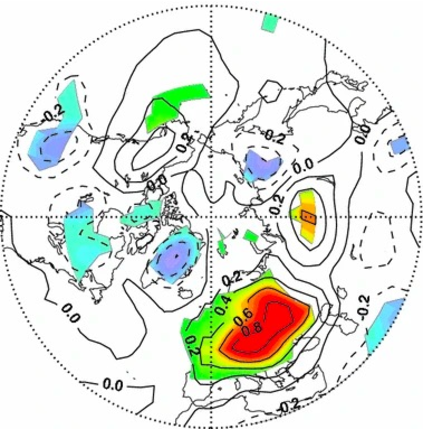
\includegraphics[scale=0.6]{master_thesis_contents/master_thesis_fig/rozanov2012_fig12.pdf}
        \subcaption{シミュレーション結果(最大で$0.8\, \mathrm{K}$の増加、~\cite{rozanov2012influence}より引用)}
        \label{fig:rozanov2012_fig12}
    \end{minipage}
    \begin{minipage}{\linewidth}
        \centering
        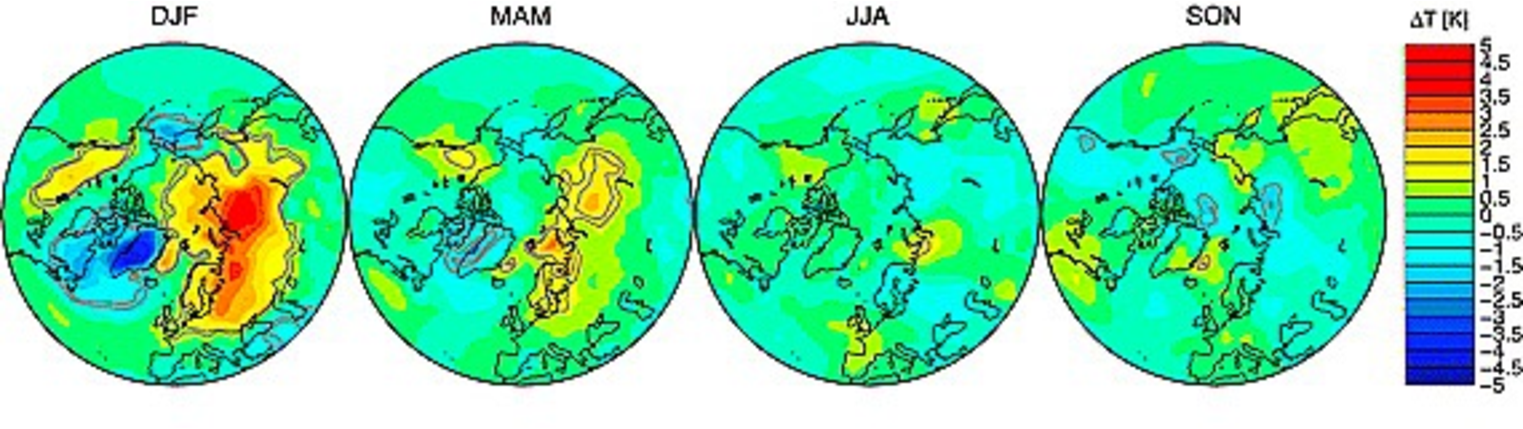
\includegraphics[scale=0.6]{master_thesis_contents/master_thesis_fig/seppala2009_fig3.pdf}
        \subcaption{観測データに基づいた統計結果(最大で$5\, \mathrm{K}$の増加、~\cite{seppala2009geomagnetic}より引用)}
        \label{fig:seppala2009_fig3}
    \end{minipage}
    \caption{EPP時の地表温度の変化$\Delta T\, \mathrm{[K]}$(シュミレーション結果と観測結果の両方に地表温度の上昇が確認できるが、上昇のピークの値に差がある)}
    \label{fig:rozanov2012_seppala2009}
\end{figure}
そこで我々の研究グループでは、EPPの影響による\ce{O3}の変動を観測的に明らかにすることを目的の1つとして研究を行っている。
EPPの影響による\ce{O3}の変動は、図\ref{fig:epp_to_ozone_flow}のようなシナリオが考えられている~\cite{rozanov2012influence}。
\begin{figure}[htbp]
    \centering
    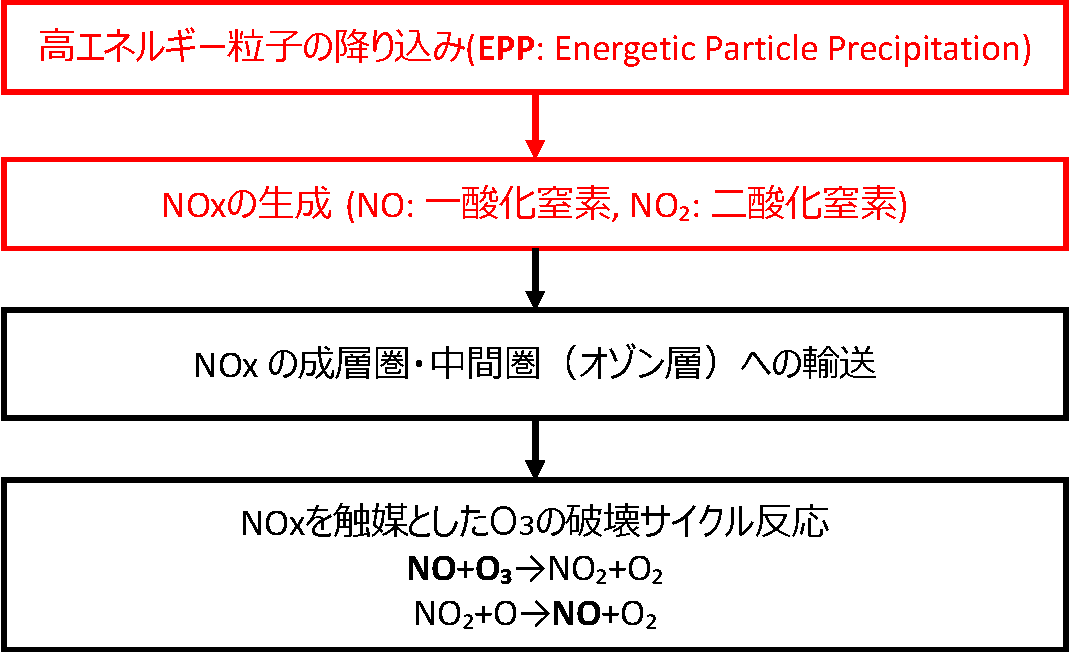
\includegraphics[width=\linewidth]{master_thesis_contents/master_thesis_fig/epp_to_ozone_flow.pdf}
    \caption{EPPから\ce{O3}破壊までのフロー}
    \label{fig:epp_to_ozone_flow}
\end{figure}
まずEPPが起きると、それによって上部中間圏〜熱圏の高度で$\mathrm{NO}_x$と呼ばれる一酸化窒素\ce{NO}や二酸化窒素\ce{NO2}が生成される。
それが大気の鉛直輸送によって成層圏・中間圏に輸送されることにより、図\ref{fig:rozanov2012_seppala2009}の反応式で表されるように\ce{O3}の破壊サイクル反応を起こす。


\section{先行研究の結果と課題}
\label{sec:intro_privious}
先行研究ではEPPによって$\mathrm{NO}_x$が増加し、それが\ce{O3}の変動に影響を与えていることがMIPASによる衛星観測のデータにて時間分解能が1日ではあるが示されている(図\ref{fig:lopez2005observation_fig3})~\cite{lopez2005observation}。
2003年10月28日にEPPがあったが、その後に$\mathrm{NO}_x$の増加が確認されており、$\mathrm{NO}_x$の増加があった領域において\ce{O3}の減少が確認できる。
\begin{figure}[htbp]
    \centering
    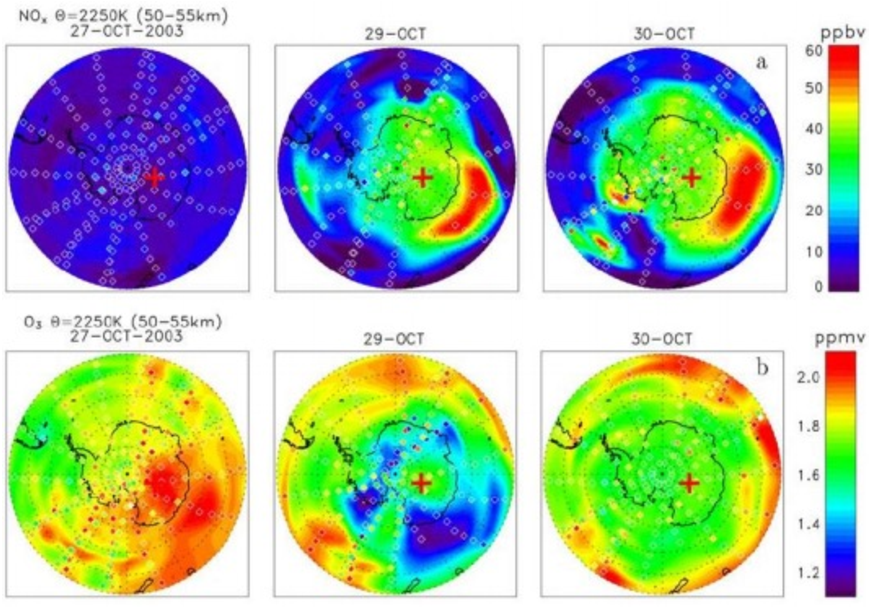
\includegraphics[width=\linewidth]{master_thesis_contents/master_thesis_fig/lopez2005observation_fig3.pdf}
    \caption{EPPイベントの前後での南半球の高度$50-55\, \mathrm{km}$における$\mathrm{NO}_x$と\ce{O3}の変動(~\cite{lopez2005observation}より引用)}
    \label{fig:lopez2005observation_fig3}
\end{figure}
MIPASは太陽同期軌道を周回する衛星であり、リム観測で大気分子観測を行う衛星である。
このような衛星観測はこの図で示されるように全球的な観測を行うことには向いているが、衛星軌道の特性により時間分解能は1日と比較的悪く、ある一地点における高時間分解能かつ連続的な観測には向いていないという課題があった。
その課題を克服するため、我々の研究グループではミリ波分光計(観測手法の詳細は\ref{ch:mm_obs}章で述べる)を用いた観測を行っている。\par
ミリ波分光を用いた地上観測と衛星観測は相補的な関係にあるため、必要に応じて衛星観測のデータを補足的に用いる。
% 修正済
% どちらが優れているとか、ミリ波観測があれば衛星観測は不要、という主張に受け取られないように、それらの観測は相補的であるという文章があると良い。
次に、我々の研究グループが行ったミリ波分光計を用いたこれまでの研究について紹介する。
我々は、2011年から南極昭和基地でミリ波分光計による\ce{O3}と\ce{NO}の地上観測を行っている。
図\ref{fig:isono2014ground_fig5a}は、2012年から2013年までの観測による\ce{NO}の柱密度の時間変動の結果である~\cite{isono2014ground}。
横軸が時系列になっていて、エラーバー付きのプロットは\ce{NO}の柱密度を示しており1日1プロットである。
背景の紫色の影の部分は、高度$100\, \mathrm{km}$におけるそれぞれの日で太陽が当たっていない時間の長さを表している。
この結果より、季節変化にともなう長期的な変動のほか、冬期(4月〜8月頃)には4日程度の顕著な短期的変動が確認できた。
この短期的な変動は、EPPにともなう現象であると考えられる。
しかし一方で、\ce{NO}は光解離するため、夏(10月〜翌年2月頃)においては太陽光による影響も考慮に入れる必要がある。
そのため、夏においてはEPPイベントの際に、\ce{NO}の増加と、光解離による\ce{NO}の減少が同時に起きるため、光解離の影響とEPPの影響は切り分けることができなかった(図\ref{fig:isono2014ground_fig5a}の紫色の影の部分がない時期のプロット。エラーバーの範囲を超えた顕著な短期変動は確認できない)。
\begin{figure}[htbp]
    \centering
    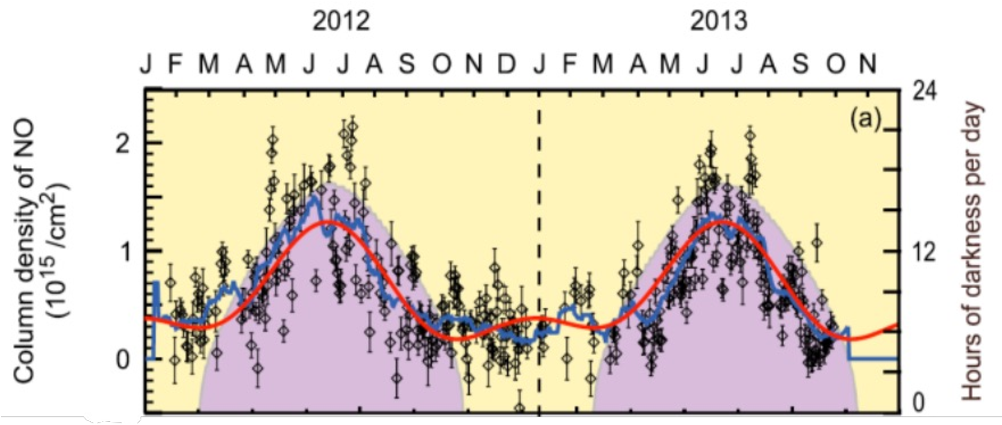
\includegraphics[width=\linewidth]{master_thesis_contents/master_thesis_fig/isono2014ground_fig5a.pdf}
    \caption{ミリ波分光計を用いた観測による南極・昭和基地での\ce{NO}の変動(エラーバー付きのプロットは\ce{NO}の柱密度を示しており1日1プロットである。
    紫色の影の部分は、高度$100\, \mathrm{km}$におけるそれぞれの日で太陽が当たっていない時間を表している。青色の線は31日間の移動平均、赤色の線は年周期成分と半年周期成分からなる正弦波によるフィッティングを行ったもの。~\cite{isono2014ground}より引用)}
    \label{fig:isono2014ground_fig5a}
\end{figure}
以上のことを踏まえて、先行研究での衛星観測とミリ波分光計での地上観測で明らかになったことと、それらの課題点についてまとめる。
\clearpage
\begin{itemize}
    \item 明らかになった点
    \begin{itemize}
        \item ミリ波分光を用いた地上観測(南極・昭和基地)
        \begin{itemize}
            \item 季節にともなう\ce{NO}の長期的変動
            \item EPPに伴う\ce{NO}の増加
        \end{itemize}
        \item 衛星観測
        \begin{itemize}
            \item EPPに伴う高度$50\, \mathrm{km}$付近のグローバルな\ce{NO}の増加
            \item \ce{NO}の増加した領域での\ce{O3}の減少
        \end{itemize}
    \end{itemize}
    \item 課題点
    \begin{itemize}
        \item ミリ波分光計を用いた地上観測(南極・昭和基地)
        \begin{itemize}
            \item 夏の\ce{NO}の短期変動の確認が難しい
        \end{itemize}
        \item 衛星観測
        \begin{itemize}
            \item 定点での連続的な観測が難しい
        \end{itemize}
    \end{itemize}
\end{itemize}
\ref{sec:intro_porpose}節では、これらの課題点を踏まえた本研究の目的について述べていく。


\section{本研究の目的と研究手法}
\label{sec:intro_porpose}
本研究では、図\ref{fig:epp_to_ozone_flow}で示したEPPによる\ce{O3}破壊現象のフローの中で、まずは上の2つの関係の解明に取り組んだ(図\ref{fig:flow_and_porpose}中の赤枠)。
EPPについては、Dst指数と呼ばれる地磁気擾乱の大きさを表す指数と衛星観測による電子フラックスデータから現象の同定を行い、その規模などの特性を調べた。
加えて、NASAが提供しているOMNI Web Dataを用いて、電子フラックスの増加の原因となる事象が何かを調べた。
$\mathrm{NO}_x$については、ミリ波観測による\ce{NO}のスペクトルデータから柱密度を導出し、その時間変動について調べた。
最後に、これらの関係性について調べることにより、EPPがどのように\ce{NO}の変動に影響を与えているかについて明らかにする。
\begin{figure}[htbp]
    \centering
    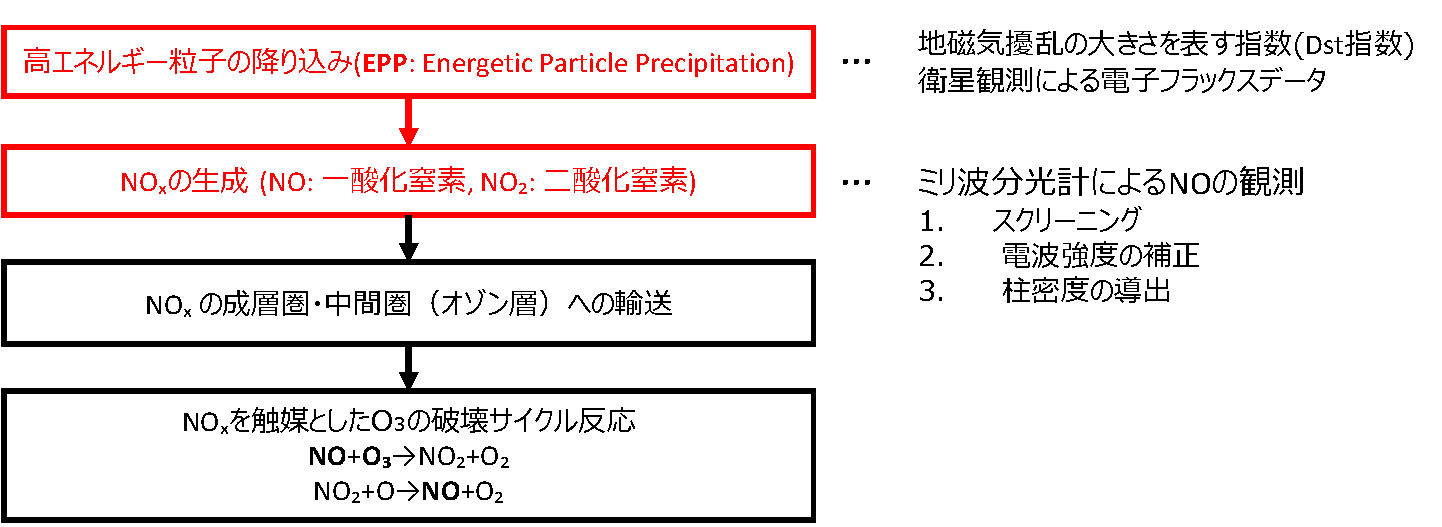
\includegraphics[width=\linewidth]{master_thesis_contents/master_thesis_fig/flow_and_porpose.pdf}
    \caption{EPPによる\ce{O3}破壊現象の流れと本研究の目的・手法との対応}
    \label{fig:flow_and_porpose}
\end{figure}
